\documentclass{article}
%\documentclass[a4paper,12pt,twoside,brazil]{article}

\usepackage[top=25mm,bottom=20mm,left=20mm,right=25mm]{geometry} %coloca o
% tamanho das margens
\usepackage[T1]{fontenc}        % pacote para conj. de caracteres correto
\usepackage[utf8]{inputenc}     % pacote para acentuação
\usepackage[brazil]{babel}

\usepackage{graphicx}           % pacote para importar figuras
\usepackage{times}              % pacote para usar fonte Adobe Times
\usepackage{mathptmx}           % p/ usar fonte Adobe Times nas fórmulas
\usepackage{enumerate}
\usepackage{verbatim}
\usepackage{moreverb}
\usepackage{ulem}
\usepackage{textcomp}
\usepackage{amsmath}
\usepackage{amssymb}
\usepackage{color}
\usepackage{colortbl}
\usepackage{fancybox}
\usepackage{indentfirst} %indenta a primeira linha
\usepackage{titlesec} %para os gr\'{a}ficos dos cap\'{\i}tulos
\usepackage{textfit}
\usepackage{fancyhdr} % Para colocar cabe\c{c}alho nas p\'{a}ginas
\usepackage{subfigure}
\usepackage{lettrine} % Para fazer letras capitulares
\usepackage{lscape}
\usepackage{lmodern} % fonte CMR que funciona
\usepackage{setspace}
\usepackage{caption}
\usepackage{subcaption}

\newcommand{\foot}[1]{\footnote{	\fontfamily{cmss}\selectfont\footnotesize{#1}}}

\newcommand{\fig}[1]{\textit{Figura~\ref{#1}}}

\newcommand{\blankpage}{\newpage\thispagestyle{empty}	\mbox{}
	%\mbox{Esta página foi intencionalmente deixada em branco.}
	\newpage}
	
\begin{document}

\tableofcontents
\newpage

\onehalfspacing

\section{Resumo}

O objetivo deste trabalho é pesquisar, propor e desenvolver um sistema que
capacite um veículo terrestre a se locomover de modo autônomo em ambientes
externos não estruturados ou pouco estruturados, ou seja, em um campo com
vegetação/plantação e/ou em uma floresta pouco densa (\textit{outdoor} e
\textit{off-road}). O veículo deverá ser capaz de se dirigir até uma localização
pré-determinada (coordenada GPS) escolhendo por meios próprios o caminho a
seguir, ao mesmo tempo em que desvia de obstáculos, percebendo-os de forma
autônoma. O sistema de navegação autônoma irá se basear na aquisição e
processamento de imagens, obtidas a partir de um par de câmeras (câmera
estéreo), constituindo assim um sistema de visão binocular do qual é possível se
obter uma percepção tridimensional do ambiente. Portanto, pretende-se extrair
parâmetros de navegabilidade do ambiente percebido pela câmera estéreo, como
caminhos livres, obstruções e obstáculos, que combinados com as informações de
posição e orientação do veículo e do ponto de destino (baseando-se em
coordenadas de GPS) serão integrados em um sistema robusto de navegação.

Inicialmente serão estudados e trabalhados algoritmos para a criação do mapa de
disparidade a partir do par de imagens obtidas pela câmera estéreo.
A partir do mapa de disparidade, será elaborado um mapa local de navegabilidade
que irá processar e classificar o espaço tridimensional percebido, separando e
representando as regiões navegáveis (seguras) e as regiões não navegáveis
(obstáculos e regiões à evitar) do espaço em frente ao veículo. Este mapa local
será utilizado em conjunto com as informações de posição atual e de destino (GPS
e bússola) a fim de realizar o controle da navegação do veículo. Estão sendo
consideradas duas abordagens principais para o controle local da navegação: a
primeira baseada no uso de Redes Neurais Artificiais, conforme proposto em
trabalhos anteriores desenvolvidos por membros do grupo do LRM\foot{Laboratório
de Robótica Móvel - http://lrm.icmc.usp.br} e a segunda baseada em uma adaptação
do algoritmo VFH. Nestas abordagens serão consideradas como parâmetro de entrada
as informações tridimensionais do mapa de navegabilidade. As principais
contribuições esperadas deste trabalho são a adaptação e aperfeiçoamento dos
algoritmos para a geração de mapas de disparidade, a proposta e o
desenvolvimento de algoritmos para a obtenção de mapas locais de navegabilidade
com informações espaciais (3D), e por fim o aperfeiçoamento de técnicas
previamente desenvolvidas para detectar e desviar de obstáculos em mapas 2D, a
fim de permitir uma navegação baseada no mapa de navegabilidade 3D.



\section{Introdução}

Este documento apresenta o relatório parcial do Projeto “Navegação de Veículos
Autônomos em Ambiente Externo Não Estruturado baseada em Visão Computacional”,
com a descrição e discussão das atividades realizadas no primeiro ano de
vigência da bolsa de mestrado concedida.

A primeira etapa do projeto consiste na obtenção de dados tridimensionais a
partir de uma câmera estéreo. Está sendo utilizado como equipamentos duas
abordagens. A primeira utilizando uma câmera estéreo Point Grey Bumblebee2 que
já possui duas lentes dispostas de forma fixa permitindo um campo de visão
restrito. A outra abordagem é o uso de duas (ou três) câmeras simples do tipo
Point Grey Flea podendo serem dispostas com certa liberdade para formar o
conjunto estéreo e assim ter um campo de visão ajustado de acordo com a
necessidade. Ambas abordagens requerem uma calibração das lentes e do conjunto
estéreo, sendo a segunda abordagem mais sujeita a problemas de descalibração por
trepidações e desregulagem dos seus posicionamentos provocada pelas vibrações.

Dada a informação sensorial a partir de visão computacional a segunda etapa
consiste em transformar esta informação em uma forma estruturada para análise e
interpretação dos dados. As próximas etapas do projeto consistem em criar o mapa
de navegabilidade de forma que a informação tridimensional captada pela câmera
estéreo possa ser agregada ao planejamento de navegação autônoma do veículo.

Primeiramente o desenvolvimento está sendo efetuado em ambiente simulado. Os
experimentos em simulação serão validados no ambiente real em um cenário
limitado porém com as características definidas no projeto, ou seja, um cenário
externo não estruturado.


\section{Objetivos}


\subsection{Objetivo geral}

O objetivo geral deste trabalho é desenvolver um sistema de navegação autônoma
baseado em visão computacional a fim de capacitar um veículo terrestre autônomo
a se locomover em ambientes externos não estruturados, ou seja, em campos com
vegetação/plantação e/ou em florestas pouco densas. O veículo deverá ser capaz
de se dirigir até uma localização determinada, desviando dos obstáculos,
percebendo-os de forma autônoma, e escolhendo por meios próprios o caminho a
seguir. O veículo autônomo deverá ter a capacidade de identificar os elementos
do terreno onde irá se deslocar, identificando o chão e os obstáculos, a fim de
evitar zonas não transponíveis ou muito acidentadas. Portanto, o objetivo deste
trabalho é desenvolver um sistema de navegação robusto e seguro voltado à
aplicação em veículos autônomos para ambientes externos não estruturados (ou
muito pouco estruturados), baseado no uso de visão computacional realizada
através da captura de imagens estéreo, no uso de mapas de profundidade (mapas de
disparidade), e no uso mapas locais de navegabilidade.

\subsection{Objetivos Específicos}

Os principais objetivos específicos deste projeto de mestrado, que se apresentam
como um desdobramento do objetivo geral descrito acima, são:

\begin{itemize}

\item Extração de referenciais a partir de um par de câmeras, constituindo um
sistema de visão binocular (estéreo);

\item Propor melhorias nos algoritmos de geração do mapa de disparidade, obtido
a partir das imagens estéreo;

\item Gerar um mapa de navegabilidade local a partir de informações visuais;

\item Desenvolver um mecanismo de navegação autônoma, baseado nas informações de
GPS, Bússola e do Sistema de Visão, capaz de desviar de obstáculos e dirigir o
veículo até um destino determinado de forma robusta e eficiente;

\item Fazer uso dos conhecimentos prévios de trabalhos desenvolvidos no
laboratório e contribuir para a consolidação de tecnologias capazes de atribuir
navegabilidade autônoma a veículos de diversas naturezas para fins práticos;

\item Aplicação e avaliação do sistema de navegação autônoma em um veículo real
em ambiente externo não estruturado.

\end{itemize}



\section{Atividades acadêmicas}

Foram concluídas as disciplinas do mestrado contabilizando 58 créditos (sendo
48 obrigatórios) todas com conceito de aprovação \textbf{A}. Também, a aprovação
no exame de proficiência em inglês e no exame de qualificação exigidos pelo programa de
pós-graduação.\\

\textbf{Disciplinas cursadas:}
\begin{itemize}
\item Projeto de Algoritmos
\item Introdução aos Sistemas Evolutivos
\item Introdução aos Sistemas Embarcados
\item Introdução aos Sistemas Robóticos
\item Preparação Pedagógica
\item Algoritmos de Estimação para Robótica Móvel
\item Robôs Móveis Autônomos
\item Metodologia de Pesquisa Científica em Inteligência Artificial
\item Algoritmos de Estimação de Distribuição
\end{itemize}

\textbf{Participação dos seguintes eventos:}
\begin{itemize}
\item 3a. Escola Luso-Brasileira de Computação Evolutiva – ICMC / USP – 2 a 5 de
Abril de 2012;
\item 2a. Conferência Brasileira em Sistemas Embarcados Críticos – CBSEC –
Campinas/SP – 21 a 25 de Maio de 2012;
\item I Feira de Inovação e Empreendedorismo - EACH / USP - 23 a 25 de Agosto de
2012;
\item Workshop on Probabilistic and Statistical Methods - ICMC / USP - 28, 29,
30 de Janeiro de 2013.
\end{itemize}

\subsection{Participação em publicações}

Durante o primeiro ano do mestrado foram efetuados alguns trabalhos em conjunto
com colegas dos quais resultaram na participação em dois artigos submetidos:\\

\\

\textit{Patrícia A. Vargas; Gustavo Pessin; Daniel O. Sales; Maurício A. Dias;
Rafael L. Klaser; Fernando S. Osório},
Applying Swarm Intelligence to a Garbage and Recycling Collection Problem.,
\textbf{Soft computing}, (Submetido em: Dezembro de 2012)
\\

\textit{Leandro C. Fernandes; Jeferson R. Souza; Gustavo Pessin; Patrick Y.
Shinzato; Daniel Sales; Caio Mendes; Marcos Prado; Rafael Klaser; André Chaves
Magalhães; Daniel Pigatto; Kalinka Castelo Branco; Valdir Grassi Jr.; Fernando
S. Osório; Denis F. Wolf},
CaRINA Intelligent Robotic Car:
Architectural Design and Implementations., \textbf{Journal of System
Architecture}, (Submetido em: Janeiro de 2013)




\section{Detalhamento}


Uma das necessidades básicas para a navegação autônoma é o conhecimento da
localização do veículo. Para esta localização a odometria do veículo tem papel
importante em informar o deslocamento e pose do veículo durante o seu movimento.
A abordagem para a localização do veículo neste projeto é através do uso do GPS,
que também é possível obter os dados de odometria a partir deste sensor. Um dos
problemas associados ao GPS é a localização mais precisa em pequenos
deslocamentos como manobras de desvio de obstáculos. Já uma odometria baseada em
encoder nas rodas do veículo permitem uma odometria mais precisa nestas
condições, porém diverge rapidamente em maiores distâncias. A abordagem que está
sendo considerada é a integração das duas odometrias (pelo encoder e pelo GPS)
através de um filtro estendido de Kalman que estima e atualiza a odometria.

Foram efetuados experimentos com a odometria baseada em encoder na plataforma
CaRINA I que levaram à necessidade de melhorias neste módulo do veículo. Foi
desenvolvido um novo módulo de odometria baseado no encoder da roda e da barra
da direção integrado com os dados da unidade de medida inercial (IMU) que está
sendo utilizada no projeto. O novo módulo também tem ajustes no calculo da
geometria Ackermann levando em consideração as 4 rodas do veículo resultando em
uma melhor estimação da odometria.


Para este trabalho a simulação desempenha um papel essencial nos testes e na
avaliação das técnicas a serem utilizadas. Para tal está sendo utilizada a
plataforma ROS\foot{ROS - Robotic Operating System - http://wqww.ros.org} que
possui o simulador físico 3D Gazebo. Esta plataforma está sendo considerara por
estar sendo adotada por diversos grupos de pesquisa na área da robótica. É uma
plataforma \textit{Open Source} que também tem servido de repositório para
compartilhar implementações de algoritmos propostos pela comunidade científica,
assim como \textit{drivers} de acesso aos dispositivos físicos, como sensores e
até mesmo plataformas robóticas completas (ex.
PR2\foot{PR2 - Personal Robot 2 - http://www.willowgarage.com}).


Para a modelagem em ambiente simulado foi feito o levantamento com o veículo
real dos parâmetros dos sensores - câmera estéreo, imu, gps, encoders - que
foram utilizados para criar o modelos destes sensores no simulador.\foot{Vídeo:
http://www.youtube.com/watch?v=deF\_QIhFNtM}


A modelagem do sistema em um ambiente virtual é um passo fundamental para
executar experimentos em um simulador. Os experimentos em simulação podem ser
replicados e repetidos mais facilmente, desta forma, uma maior quantidade de
dados pode ser extraída para análises e verificação do comportamento dos
algoritmos. A maioria dos algoritmos utilizados no contexto da robótica móvel
autônoma requerem uma parametrização e um refino de diversos parâmetros para se
adequarem às necessidades da aplicação. Este refino está diretamente associado
aos comportamentos desejados que devem ser testados. Com o uso de simulação
estes parâmetros e seus efeitos podem ser melhor observados antes de se levar o
experimento para o ambiente real.

Para a plataforma CaRINA I\foot{CaRINA I -
http://http://lrm.icmc.usp.br/?page=projetos&projeto=carina} que será utilizada
já foram descritos os modelos de simulação, do veículo e de alguns cenários de
testes (\fig{fig:model}, \fig{fig:gazebo}).

\begin{figure}[ht]
	\begin{minipage}[b]{0.4\linewidth}
	    \centering
	    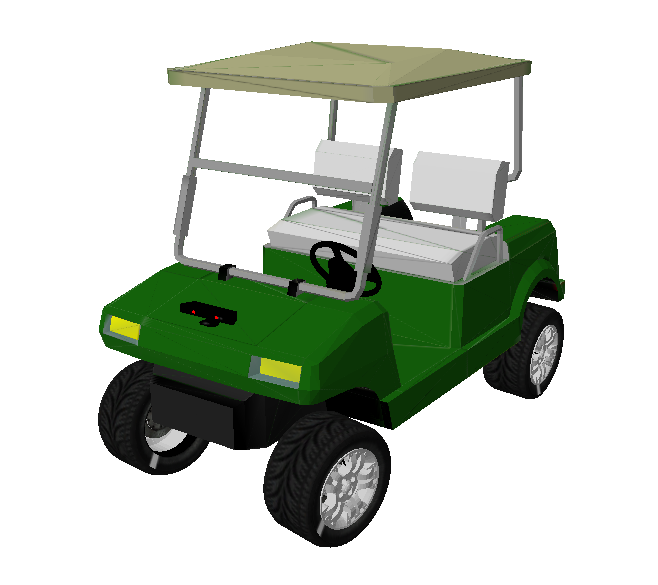
\includegraphics[width=8cm]{../images/carina_rviz_fundo_branco_sem_grid.png}
	 	\caption{CaRINA I - modelo virtual}
	 	\label{fig:model}
	\end{minipage}
	\hspace{1cm}
	\begin{minipage}[b]{0.4\linewidth}
	    \centering
	    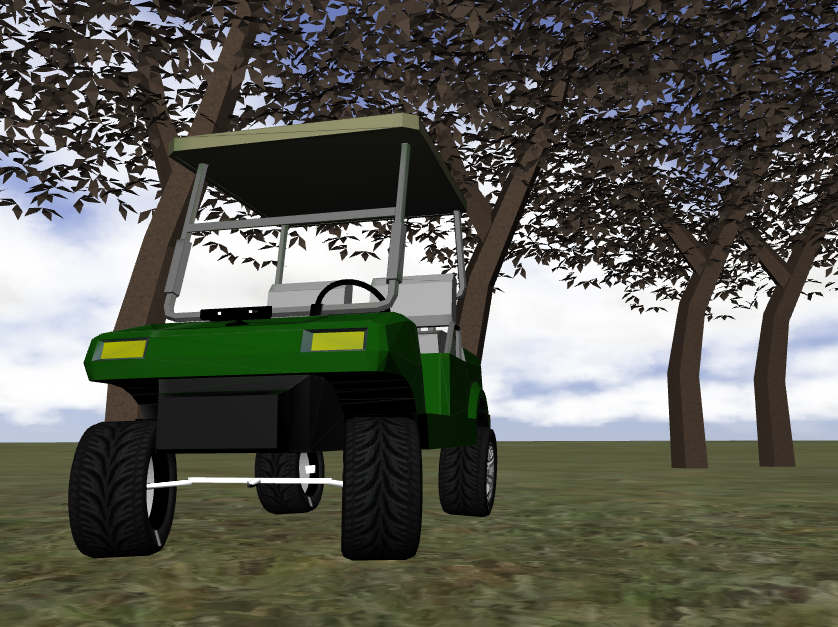
\includegraphics[width=8cm]{../images/carina_gazebo_frente_fundo.png}
	 	\caption{CaRINA I - cenário de ambiente não estruturado}
	 	\label{fig:gazebo}
	\end{minipage}
\end{figure}

Para a modelagem de robôs na plataforma ROS é utilizada uma linguagem para a
descrição chamada URDF (\textit{Unified Robot Description Format}). O URDF é
uma linguagem de descrição em XML onde basicamente são informadas os componentes,
sensores e relações entre as partes do robô, cada qual tendo um sistema de
coordenadas próprio. Estas relações podem ser móveis ou fixas, determinando
assim transformações entre cada sistema de coordenada. Toda informação sensorial
e de controle está associada a origem do seu sistema de coordenadas.





\subsection{Arquitetura}

Para o desenvolvimento do sistema e execução no ambiente real também será
utilizada a plataforma ROS, pois ela foi elaborada tendo como um dos propósitos
a padronização de uma interface para dispositivos reais e simulados. Isto
permite o desenvolvimentos dos algoritmos de forma independente da fonte dos
dados.

A arquitetura do sistema de navegação será baseado no modelo geral do ROS
conforme a \fig{fig:arq}.

\begin{figure}[!h]
  	\centering
    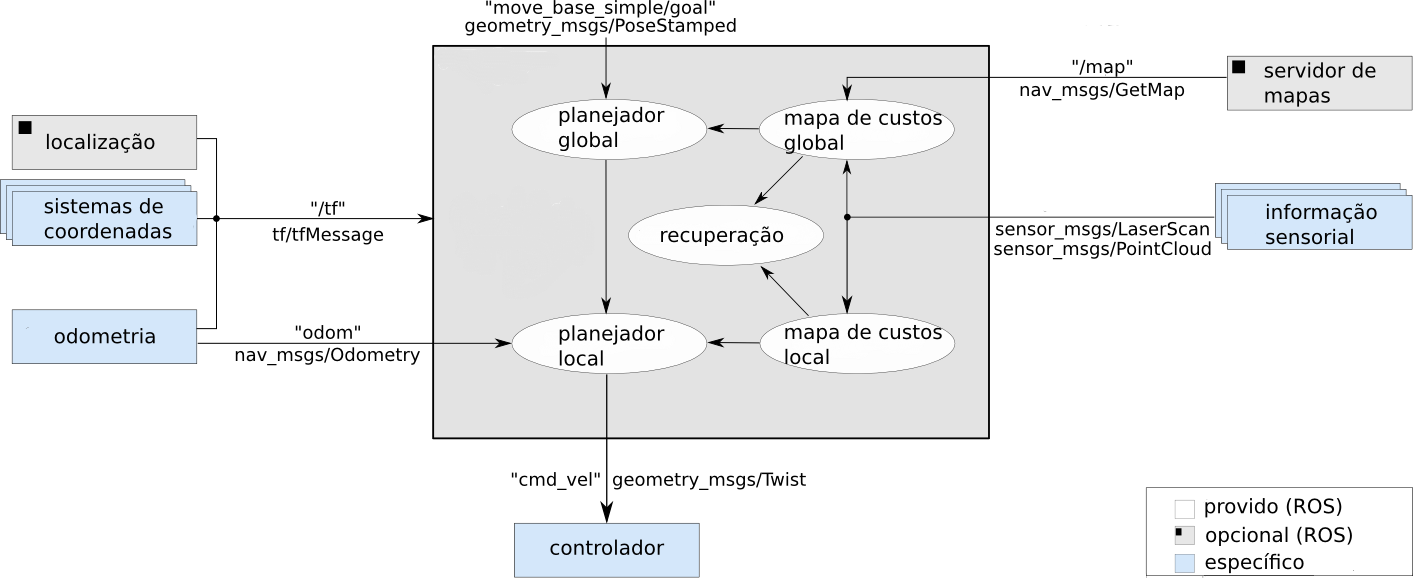
\includegraphics[width=\textwidth,height=8cm]{../images/overview_tf_pt.png}
 	\caption{Arquitetura geral do sistema de navegação.}
	\fonte{adaptado de: www.ros.org}
 	\label{fig:arq}
\end{figure}

Esta arquitetura se baseia em um comportamento deliberativo em relação ao
mapeamento global e um comportamento reativo associado ao mapeamento local. O
serviço de mapa deve fornecer informações de ocupação do espaço, geralmente
discretizado em livre, ocupado e desconhecido. Estes atributos são utilizados no
cálculo dos custos utilizado pelo algoritmo de geração de trajetória. Estes
custos são mantidos pelos mapas de custos e atualizados de acordo com as
informações sensoriais que são constantemente analisadas.

Nesta arquitetura os componentes específicos dizem respeito ao veículo e
sensores utilizados. Já os componentes providos pela plataforma ROS requerem as
devidas parametrizações e a escolha dos algoritmos adequados para o problema que
ainda estão sendo estudados.

Os módulos específicos da arquitetura já foram desenvolvidos, tanto para o
ambiente real como para o ambiente simulado. O pontos da arquitetura que ainda
estão em desenvolvimento se concentram nos mapas de custos (local e global) que
definem as áreas navegáveis e não navegáveis.


\subsection{Desenvolvimento}


\subsubsection{Odometria e Localização por GPS}

A odometria e localização é efetuada com uso de GPS e de um encoder na roda do
veículo. O GPS está sendo simulado em ambiente virtual assim como o encoder,
sendo que a odometria e localização nos ambientes real e simulado são
equivalentes.\foot{Vídeo: http://www.youtube.com/watch?v=rUFdw6cYkH0}

\begin{figure}[!h]
  	\centering
    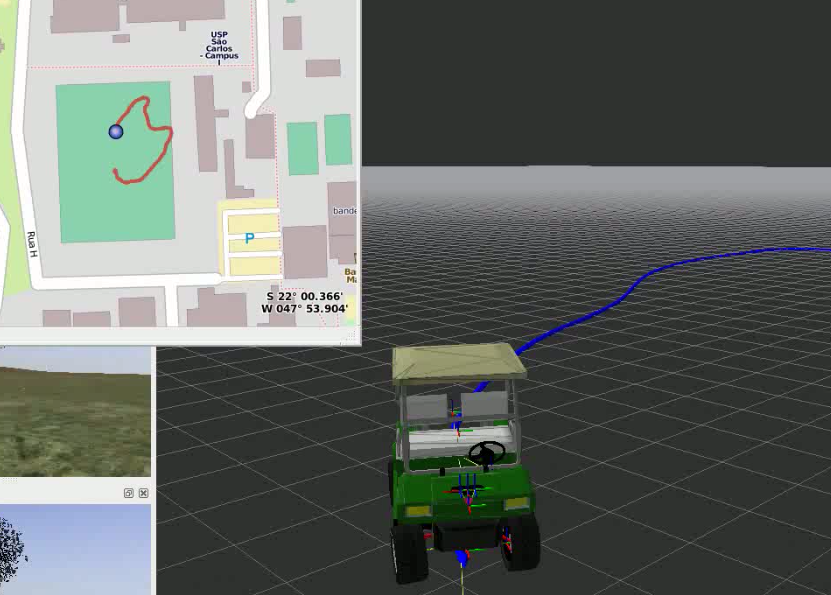
\includegraphics[width=10cm,height=7cm,]{../images/arq_odogps.png}
 	\caption{Odometria e GPS em ambiente simulado}
 	\label{fig:odogps}
\end{figure}

\subsubsection{Cálculo da disparidade}

Nesta etapa é efetuado o cálculo da disparidade entre os pixeis das imagens
relacionadas. A principal dificuldade deste cálculo é fazer a correspondência
entre cada pixel, isto é, verificar qual pixel em cada imagem
corresponde ao mesmo ponto na cena. Algoritmos que fazem esta busca são de forma
geral classificados como busca local, semiglobal e global, onde o custo
computacional tende a ser maior nos métodos globais. Foram testados dois
métodos, um local e um semiglobal. O método local Block Matching tem se
demonstrado suficiente para gerar a disparidade com um custo computacional que
permite aplicação em tempo real (\fig{fig:virt}, \fig{fig:disp}).


\begin{figure}[ht]
	\begin{minipage}[b]{0.4\linewidth}
	    \centering
	    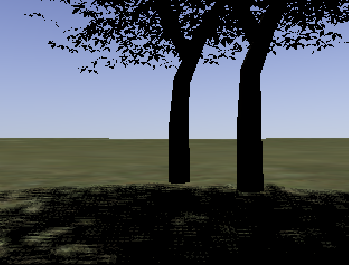
\includegraphics[width=8cm,height=7cm,]{../images/arq_image.png}
	 	\caption{Imagem obtida pela câmera estéreo (somente direita)}
	 	\label{fig:virt}
	\end{minipage}
	\hspace{1cm}
	\begin{minipage}[b]{0.4\linewidth}
	    \centering
	    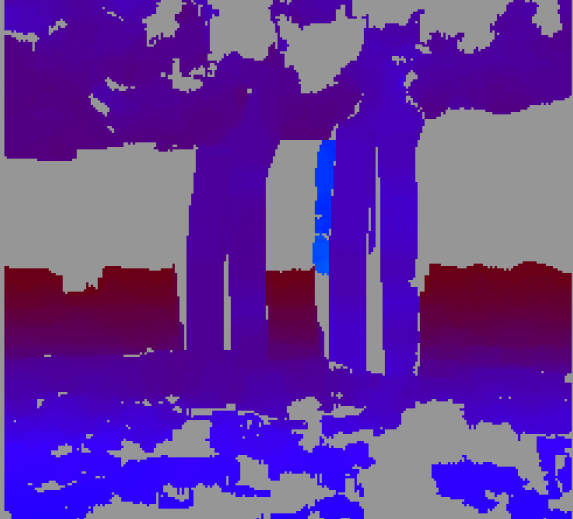
\includegraphics[width=8cm,height=7cm,]{../images/arq_disp.png}
	 	\caption{Cálculo da disparidade entre as imagens (esquerda / direita)}
	 	\label{fig:disp}
	\end{minipage}
\end{figure}


\subsubsection{Nuvem de pontos}

Uma nuvem de pontos é construída a partir das disparidades calculadas no passo
anterior. Enquanto a disparidade é apenas uma distancia relativa em pixeis de
cada ponto correlacionado, a nuvem de pontos fornece a informação tridimensional
métrica da posição do ponto no espaço. Porém, a nuvem de pontos é uma
representação não estruturada dos dados da cena, sendo então necessário uma
forma de armazenar e fazer buscas nestes dados de forma estruturada
(\fig{fig:cloud}).\foot{Vídeo: http://www.youtube.com/watch?v=MrTNStg4kc0}

\begin{figure}[!h]
  	\centering
    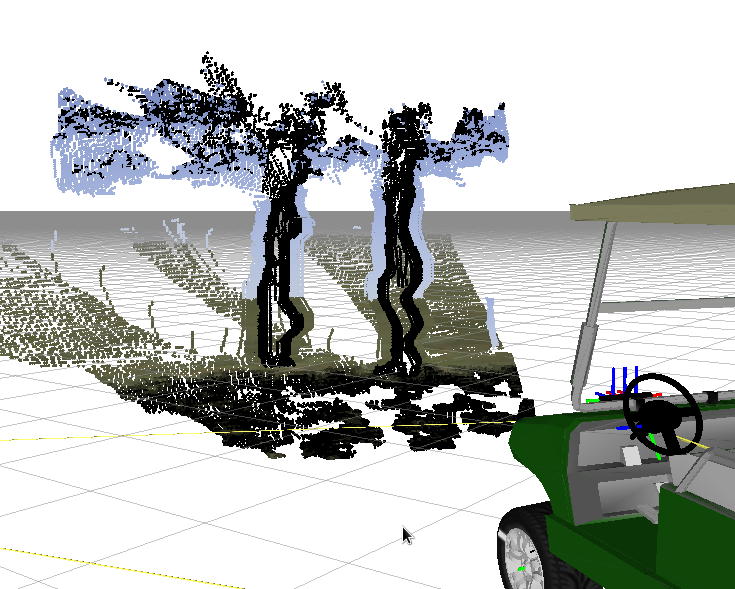
\includegraphics[width=10cm,height=7cm,]{../images/arq_cloud.png}
 	\caption{Nuvem de pontos}
 	\label{fig:cloud}
\end{figure}


\subsubsection{Octree - Discretização/Agrupamento}

A representação da nuvem de pontos em uma octree permite uma noção agrupada
dos dados assim como uma relação entre pontos vizinhos em uma estrutura em
forma de árvore. Desta forma já é possível analisar os dados de forma
estruturada e o armazenamento da informação também se torna mais reduzido devido
ao agrupamento feito pela octree discretizando o espaço em volumes cúbicos de
tamanhos variáveis (\fig{fig:octo}).


\begin{figure}[!h]
  	\centering
    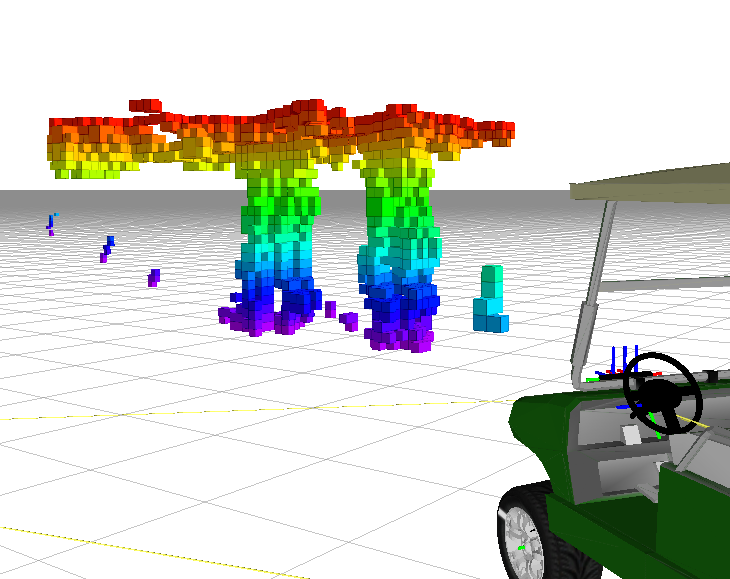
\includegraphics[width=10cm,height=7cm,]{../images/arq_octomap.png}
 	\caption{Nuvem de pontos}
 	\label{fig:octo}
\end{figure}


\subsubsection{Mapa de Ocupação / Navegabilidade}

A partir dos dados já agrupados em uma octree é possível analisar de forma
estruturada a ocupação do espaço, assim, gerando um mapa de navegabilidade
baseada na informação de ocupação ou não do espaço (\fig{fig:map}).

\begin{figure}[!h]
  	\centering
    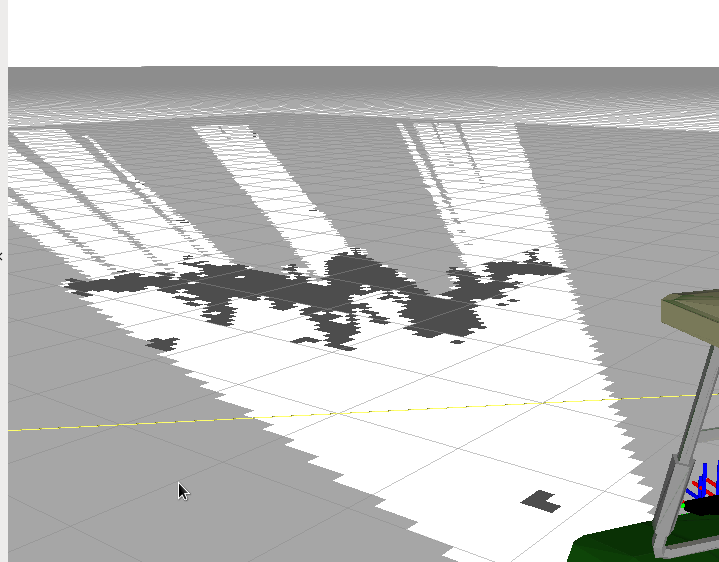
\includegraphics[width=10cm,height=7cm,]{../images/arq_mapa.png}
 	\caption{Mapa de ocupação (2D)}
 	\label{fig:map}
\end{figure}

Esta etapa ainda está sendo desenvolvida, os resultados até a presente data são
preliminares. Esta etapa concentra-se a maior atenção do projeto pois o
principal objetivo é a geração deste mapa de navegabilidade. 


\subsubsection{Próximas etapas}

As próximas etapas do projeto consistem em criar o mapa de navegabilidade de
forma que a informação tridimensional captada pela câmera estéreo possa ser
agregada ao planejamento de navegação autônoma do veículo. Este planejador
também deverá ser adaptado para contemplar as informações agregadas aos mapas de
custo.



Os experimentos em simulação serão validados no ambiente real em um cenário
limitado porém com as características definidas no projeto, ou seja, um cenário
externo não estruturado.



\section{Outros experimentos}

\subsection{Navegação e desvio de obstáculos baseados em RNA}

Este experimento basicamente foi a replicação de uma aplicação de Rede Neural
Artificial (RNA) para a navegação e desvio de obstáculos desenvolvida por um
colega do laboratório. No experimento original foi modelado um veículo com
características específicas, seguindo o modelo Ackermann. Originalmente foi
desenvolvido um simulador próprio e o treinamento de uma RNA foi efetuado em um
cenário sintético de exemplo contendo obstáculos espaçados simulando árvores. A
replicação do experimento constituiu em passar toda a modelagem para o ambiente
ROS e o simulador Gazebo já com o modelo virtual do veículo CaRINA I de acordo
com as características deste veículo. O novo cenário foi baseado no cenário
original e a rede neural utilizada foi a mesma, ou seja, não houve novo
treinamento, apenas foi aplicada ao novo cenário e o novo veículo simulando as
mesmas condições sensoriais baseada em laser. Nos testes, a rede neural
conseguiu navegar e desviar dos obstáculos de forma semelhante ao experimento
original verificando a viabilidade do uso desta técnica
(\fig{fig:robo_orig},\fig{fig:robo_gaz}).\foot{Original:
http://www.youtube.com/watch?v=vjTZzvutGEs},\foot{Vídeo:
http://www.youtube.com/watch?v=SgVab1vIB5A}

\begin{figure}[ht]
	\begin{minipage}[b]{0.4\linewidth}
	    \centering
	    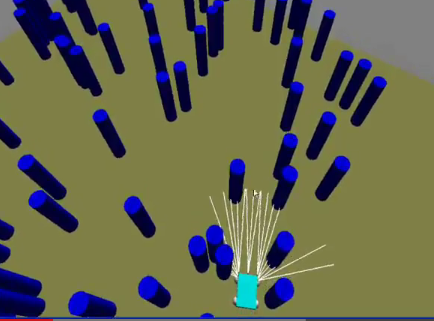
\includegraphics[width=8cm,height=7cm,]{../images/robo_orig.png}
	 	\caption{Experimento original}
	 	\label{fig:robo_orig}
	\end{minipage}
	\hspace{1cm}
	\begin{minipage}[b]{0.4\linewidth}
	    \centering
	    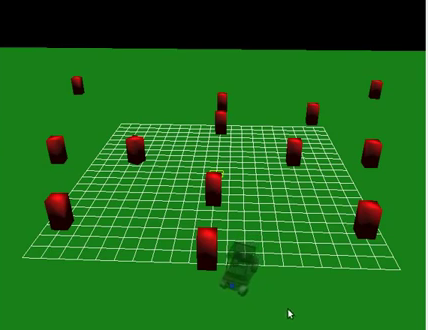
\includegraphics[width=8cm,height=7cm,]{../images/robo_gaz.png}
	 	\caption{Experimento remodelado}
	 	\label{fig:robo_gaz}
	\end{minipage}
\end{figure}


\subsection{Geração de waypoints intermediários baseado em um mapa topográfico
georeferenciado.}

Dado um mapa topográfico georeferenciado, a elevação do terreno é convertida em
custos a partir do cálculo da derivada da superfície indicando o quão íngrime é
o deslocamento de um ponto ao outro. Determinadas altitudes (altura e
profundidade) também podem ser atribuídos custos fixos elevados para inibir a
geração de um caminho nestes pontos. O algoritmo T-RRT é executado tendo como
entrada este mapa de custos, o T-RRT produz então um caminho de menor custo
indicando os pontos intermediários. Como o mapa é georeferenciados esses pontos
do caminho podem ser utilizados como waypoints de GPS intermediários para a
navegação entre pontos origem/destino distantes de forma a produzir uma
trajetória idealmente de menor dificuldade de navegação.

Esta abordagem foi testada com o propósito de avaliar o algoritmo T-RRT e
verificar a sua capacidade de gerar uma trajetória baseada em waypoints para a
navegação em áreas extensas. Pelos testes a técnica se demonstrou satisfatória
porém ainda não foi feito nenhum experimento de navegação a partir destes
resultados (\fig{fig:rrt}).

\begin{figure}[ht]
	\begin{minipage}[b]{1\linewidth}
	    \centering
	    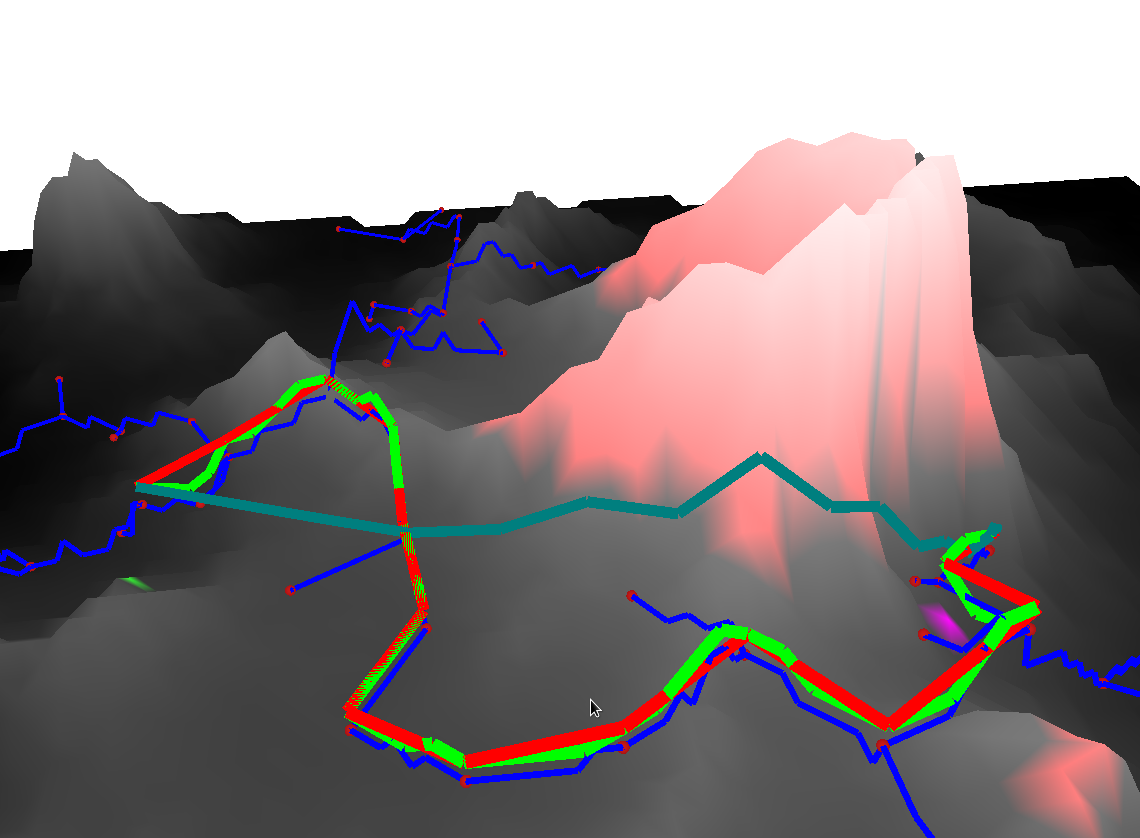
\includegraphics[width=10cm,height=6cm]{../images/rrt_2.png}
	 	\caption{Em vermelho: caminho de menor custo, Em azul: expansões, Círculos:
	 	waypoints intermediários}
	 	\label{fig:rrt}
	\end{minipage}
\end{figure}


\subsection{Navegação baseada na atração pela potência do sinal de rede wi-fi.}

No contexto deste projeto, este experimento teve como principal propósito a
familiarização com o ambiente de simulação e as ferramentas que estão sendo
utilizadas para o desenvolvimento, em destaque o ambiente ROS. Neste experimento
foi simulado o sinal de rádio de uma infraestrutura wi-fi entre antena e veículo
levando em consideração o modelo de propagação do sinal conforme norma ITU-R
P.1238. Foi desenvolvido um algoritmo simples de navegação onde o veículo é
atraído pelo aumento da potência do sinal de rádio, indicando que está se
aproximando do destino. Esta abordagem foi utilizada para validar uma estratégia
de função de fitness para métodos de otimização como PSO para navegação
autônoma. Os resultados destes experimentos foram descritos em um artigo
submetido em dezembro de 2012 (\fig{fig:path}).\foot{Vídeo:
http://www.youtube.com/watch?v=IaoADUagNj8}

\begin{figure}[ht]
	\begin{minipage}[b]{1\linewidth}
	    \centering
	    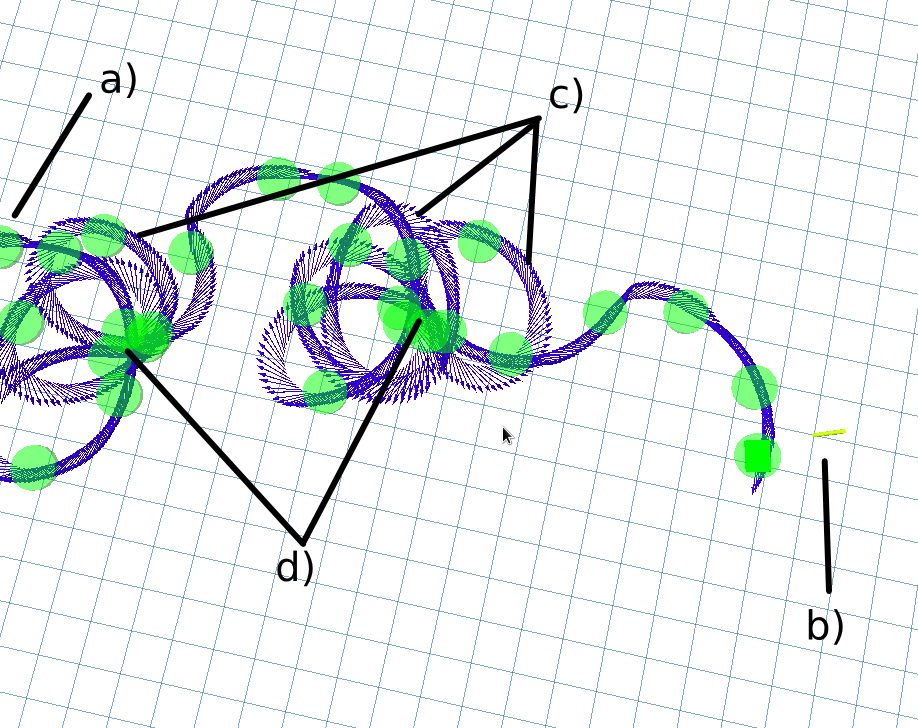
\includegraphics[width=10cm,height=6cm]{../images/beacon.png}
	 	\caption{Trajetória de navegação:
	 	a)Origem, b)Destino (antena), c)Comportamento de busca circular, d)Pontos
	 	de atração com ganho de sinal.}
	 	\label{fig:path}
	\end{minipage}
\end{figure}


\subsection{Teste de comunicação para troca de dados de GPS entre veículos.}

Estes experimentos tiveram como propósito testar a transmissão de dados de GPS
entre dois veículos utilizando a plataforma ROS. Estes testes se contextualizam
na navegação baseada em GPS onde um veículo deve seguir o outro baseado nos seus
posicionamentos fornecidos apenas pelo GPS. Os resultados dos testes se
demonstraram satisfatórios tanto na confiabilidade da comunicação como na
coerência dos dados do GPS em relação aos veículos (\fig{fig:gps_followme}).


\begin{figure}[ht]
	\begin{minipage}[b]{1\linewidth}
	    \centering
	    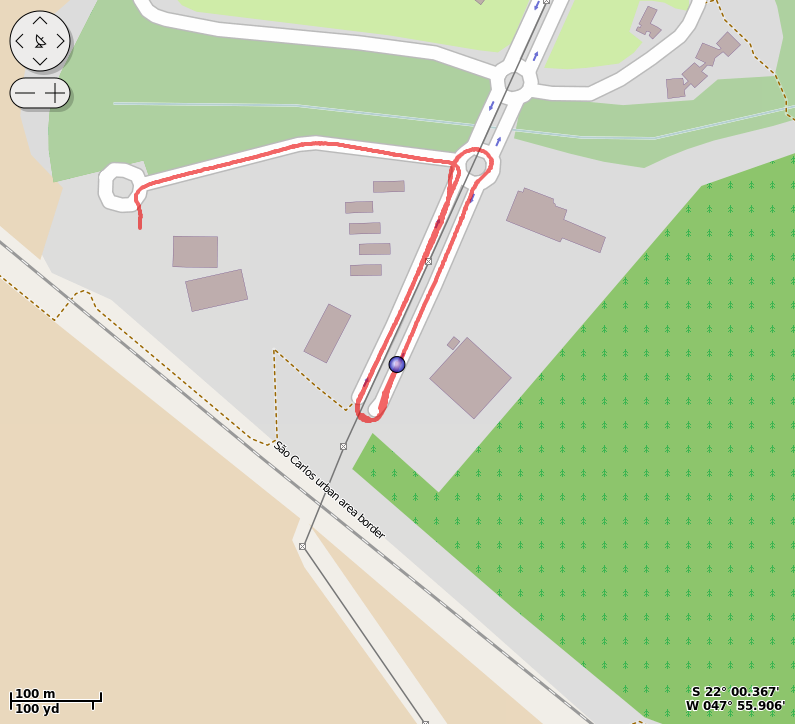
\includegraphics[width=10cm,height=6cm]{../images/gps_followme.png}
	 	\caption{Caminho dos pontos do GPS transmitidos entre veículos.}
	 	\label{fig:gps_followme}
	\end{minipage}
\end{figure}





\section{Cronograma}

O quadro abaixo apresenta um cronograma das macro atividades deste projeto. 

%A execução das mesmas se dará respeitando os devidos prazos de projeto e da
%pós-graduação que não estão aqui explicitados. A colocação temporal das macro
%atividades estão dispostas nos períodos da sua maior concentração principal,
%porém a execução das atividades se darão de forma integrada.

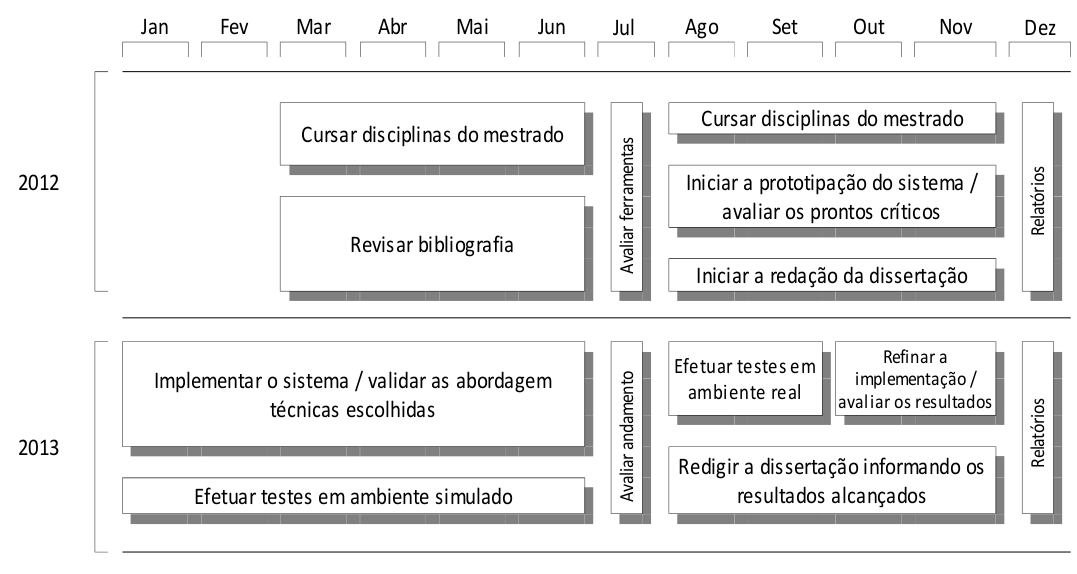
\includegraphics[width=16cm,height=8cm]{../images/chrono.png}

O projeto atualmente se encontra na fase de desenvolvimento e experimentos em
ambiente simulado e as atividades previstas estão dentro dos prazos do
cronograma.


\end{document}